\documentclass{article}

\usepackage{amsmath, amsthm, amssymb, amsfonts}
\usepackage{thmtools}
\usepackage{graphicx}
\usepackage{setspace}
\usepackage{geometry}
\usepackage{float}
\usepackage{hyperref}
\usepackage[utf8]{inputenc}
\usepackage[english]{babel}
\usepackage{framed}
\usepackage[dvipsnames]{xcolor}
\usepackage{tcolorbox}

\colorlet{LightGray}{White!90!Periwinkle}
\colorlet{LightOrange}{Orange!15}
\colorlet{LightGreen}{Green!15}

\newcommand{\HRule}[1]{\rule{\linewidth}{#1}}

\declaretheoremstyle[name=Theorem,]{thmsty}
\declaretheorem[style=thmsty,numberwithin=section]{theorem}
\tcolorboxenvironment{theorem}{colback=LightGray}

\declaretheoremstyle[name=Proposition,]{prosty}
\declaretheorem[style=prosty,numberlike=theorem]{proposition}
\tcolorboxenvironment{proposition}{colback=LightOrange}

\declaretheoremstyle[name=Principle,]{prcpsty}
\declaretheorem[style=prcpsty,numberlike=theorem]{principle}
\tcolorboxenvironment{principle}{colback=LightGreen}

\setstretch{1.2}
\geometry{
    textheight=9in,
    textwidth=5.5in,
    top=1in,
    headheight=12pt,
    headsep=25pt,
    footskip=30pt
}

% ------------------------------------------------------------------------------

\begin{document}

% ------------------------------------------------------------------------------
% Cover Page and ToC
% ------------------------------------------------------------------------------

\title{ \normalsize \textsc{}
		\\ [2.0cm]
		\HRule{1.5pt} \\
		\LARGE \textbf{\uppercase{Combinatorics Space/Time Complexity}
		\HRule{2.0pt} \\ [0.6cm] \LARGE{An analysis of the space/time complexity from resulting combinatorics graphs.} \vspace*{10\baselineskip}}
		}
\date{}
\author{\textbf{Author} \\ 
		Jack Carmichael \\
		  Andrew Burford \\
		4/19/2023}

\maketitle
\newpage

\tableofcontents
\newpage

% ------------------------------------------------------------------------------
\section{The Problem}
\label{sec:Problem}

The problem can be described from a simple scenario:
\begin{itemize}
    \item You start with a full set of items
    \item At each step, you remove one item from your current set
    \item You may continue until no items are left
    \item Once an item is removed, it cannot be added back unless you restart back to the full set
\end{itemize}
Consider all unique steps that are possible, where a step is defined as the combination of your current set and the item you choose to remove in that step. The main question of interest is how many times must you restart back to the full set in order to visit every unique step? We tackle this by first asking these questions:
\begin{enumerate}
	\item How many unique sets exist?
    \item How many unique steps exist?
    \item How many unique steps exist with respect to the number of unique sets?
\end{enumerate}

\section{Symbol Soup}
\label{sec:SymbolSoup}

This section is here for convenience to list all of the symbols that will be used. It can serve as a reference as you read the paper.

\begin{table}[h]
    \centering
    \begin{tabular}{|c|c|}
        \hline
        Symbol &  Meaning \\
        \hline
        $S$ & The initial set of items \\
        \hline
        $c$ & The total number of columns in either the graph or pascals triangle \\
        \hline
        $n_c$ & Number of nodes in column $c$, an arbitrary column \\
        \hline
        $n_t$ & Total number of nodes \\
        \hline
        $e_{n,c}$ & Number of edges coming from node $n$ in column $c$, an arbitrary node and column \\
        \hline
        $e_c$ & Number of edges in column $c$, an arbitrary column \\
        \hline
        $e_t$ & Total number of edges \\
        \hline
    \end{tabular}
    \caption{An exhaustive list of symbols that will be used in this paper.}
    \label{tab:symbolList}
\end{table}

\section{Graph Representation and Pascals Triangle}
\label{sec:GraphAndPascalsTriangle}

Before moving forward it is helpful to see the problem in the form of a graph. Figure \ref{fig:Graph} shows an example graph with an initial set, $S$, with six items, $|S|=4$.

\begin{figure}[h]
    \center
    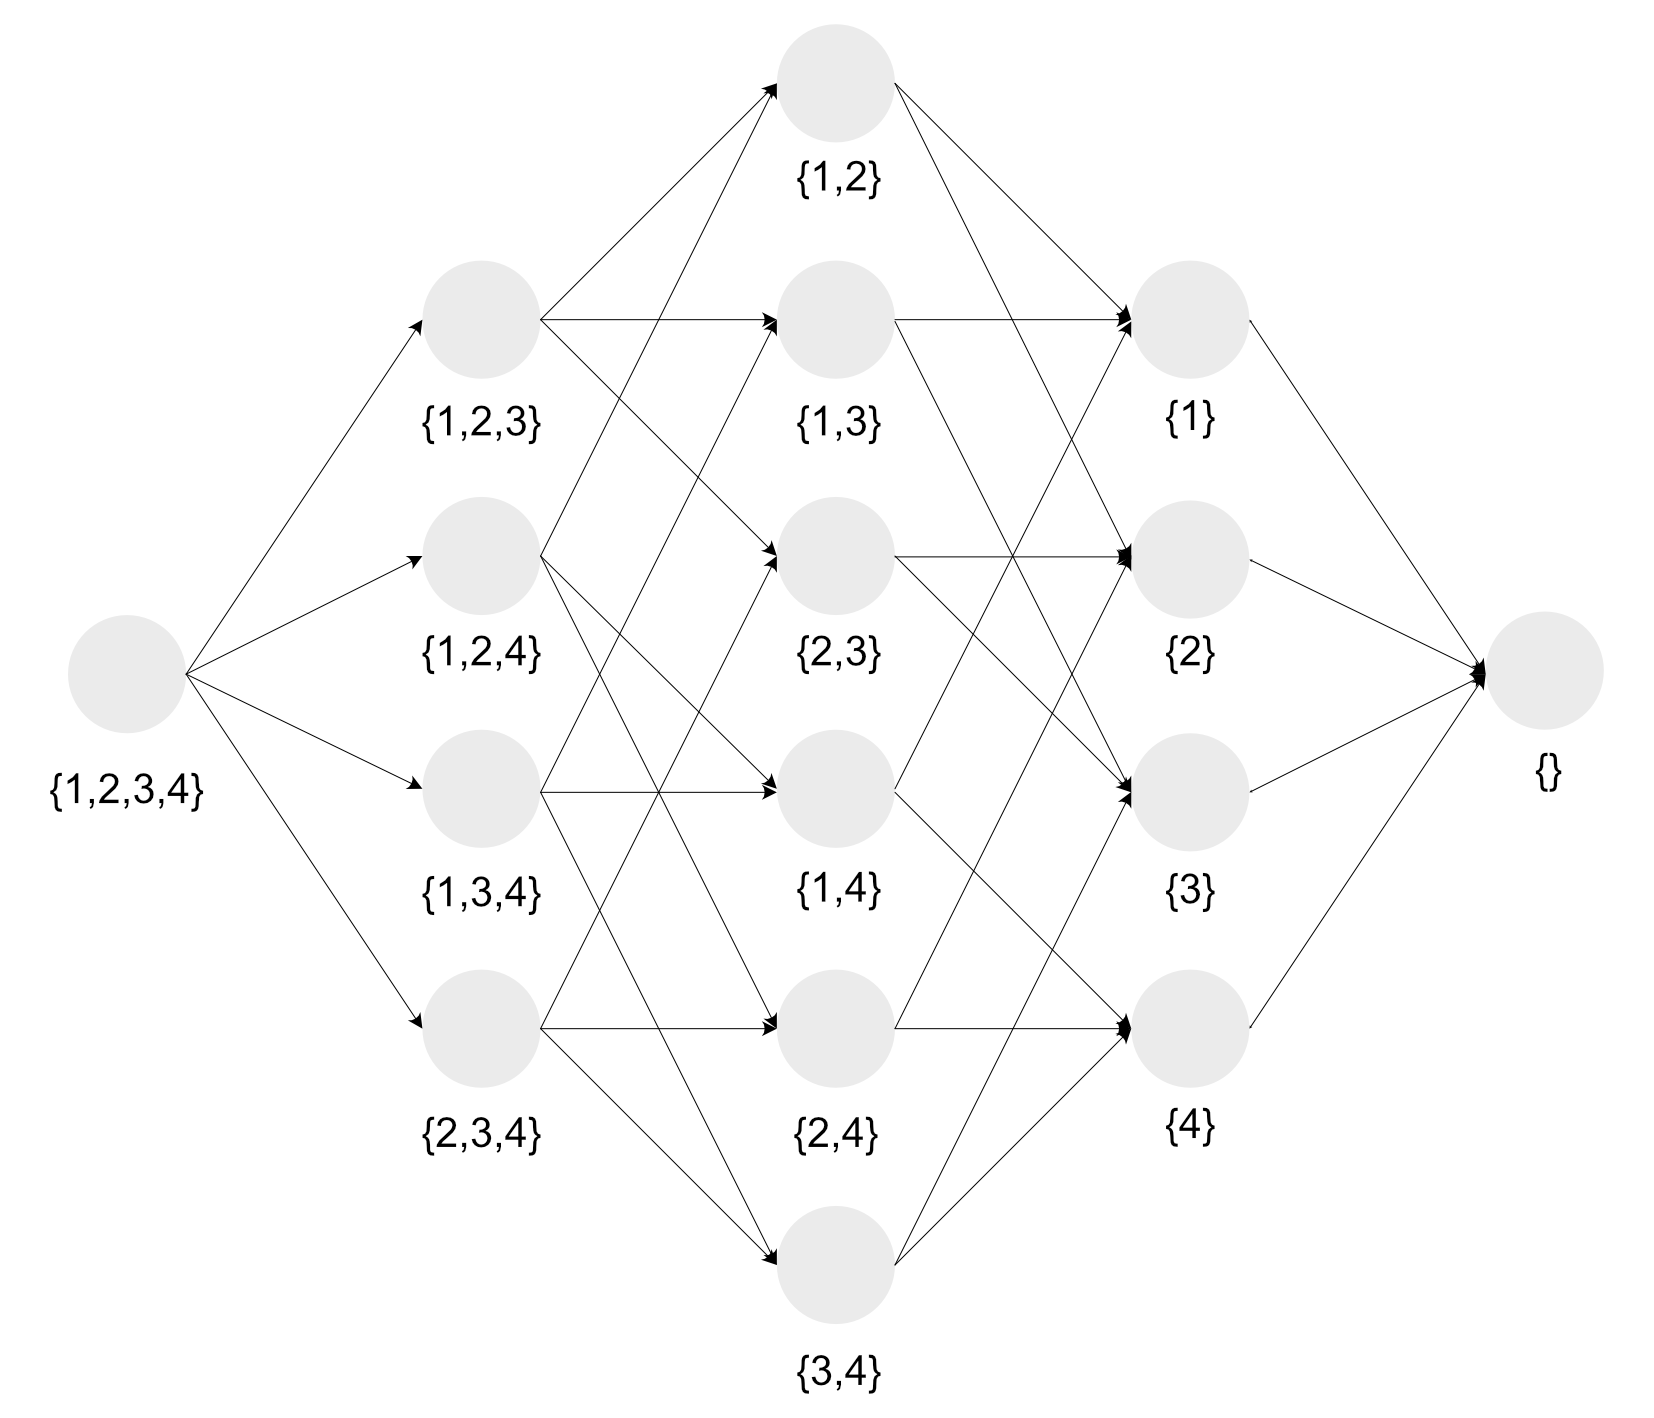
\includegraphics[scale=1]{img/Graph.png}
    \caption{The graph representation of the problem at hand. Each node represents a possible set of items.}
    \label{fig:Graph}
\end{figure}

Several things should be immediately apparent:
\begin{enumerate}
    \item The graph is symmetrical
    \item The graph closes in on itself past halfway, rather than continuing to bifurcate as a tree would.
\end{enumerate}

Beyond the initial observations, equations to represent the number of nodes and edges are needed. Once it is realized that the number of nodes in each 'column' can be calculated from a combinatoric, the equation to find the number of nodes at each column is easily found, and is shown in equation \ref{eq:NodesInColumn}. Since combinatorics are involved, pascals triangle must also be involved. Given $|S|$ flight computers, the number of columns and number of nodes in each column can be found from row $|S|+1$ of pascals triangle.

\begin{equation}
    n_c(i)=\binom{|S|}{i}=\frac{|S|!}{(|S|-i)!i!}
    \label{eq:NodesInColumn}
\end{equation}
\centerline{where $i$ is a valid column index, $c\in \{ 0\le i\le |S|\}$}

Following that, the total number of nodes in the graph can be found using equation \ref{eq:TotalNumNodes}.

\begin{equation}
    n_t=\sum_{i=0}^{|S|}n_c(i)=\sum_{i=0}^{|S|-1}\binom{|S|}{i}=\sum_{i=0}^{|S|}\frac{|S|!}{(|S|-i)!i!}
    \label{eq:TotalNumNodes}
\end{equation}

Finding the total number of edges seems to be more tricky, but the solution is to count the number of edges coming out of each node in each column. Looking at the example from figure \ref{fig:Graph}, a clear linear pattern should be apparent. This pattern can be represented using equation \ref{eq:EdgesPerNodePerColumn}.

\begin{equation}
    e_{n,c}(i)=|S|-i\\
    \label{eq:EdgesPerNodePerColumn}
\end{equation}
\centerline{where $i$ is a valid column index, $c\in \{ 0\le i\le |S|\}$}

Given this, the total number of edges in each column can be found using equation \ref{eq:EdgesPerColumn} and the total number of edges in the graph can be found using \ref{eq:TotalNumEdges}.

\begin{equation}
    e_c(i)=n_c(i)e_{n,c}(i)=\binom{|S|}{i}\left(|S|-i\right)=
    \frac{|S|!}{(|S|-i)!i!}\left(|S|-i\right)
    \label{eq:EdgesPerColumn}
\end{equation}
\begin{equation}
    e_t=\sum_{i=0}^{|S|}e_c(i)=
    \sum_{i=0}^{|S|}\binom{|S|}{i}\left(|S|-i\right)=
    \sum_{i=0}^{|S|}\frac{|S|!}{(|S|-i)!i!}\left(|S|-i\right)
    \label{eq:TotalNumEdges}
\end{equation}

With this simple analysis, the first two questions posed in section \ref{sec:Problem} are already answered. The last question requires more thought however, and it will be answered in sections \ref{sec:LowerBound}-\ref{sec:TightBound}. Before jumping right in, it may help to pose the question more mathematically. Note that the questoin can be rephrased in two ways, each one producing its own conclusion when proven.

\begin{enumerate}
    \item Given that every edge is traversed once and only once, what is the time complexity of traversing the full graph when compared to the number of nodes as $|S|\to\infty$?
    \item Given that every edge takes equal amounts of memory, what is the space used when compared to the number of nodes as $|S|\to\infty$?
\end{enumerate}

\section{Big-$\Omega$: A Lower Bound}
\label{sec:LowerBound}

The question is if the number of total number of edges grows faster or slower than the total number of nodes. In order for the total number of edges to grow slower than the total number of nodes the inequality shown in equation \ref{eq:nInequality} must be true.

\begin{equation}
    \begin{split}
        \forall i\in c\;\; \sum_{i=0}^{|S|}\frac{|S|!}{(|S|-i)!i!}(|S|-i) & \ge \sum_{i=0}^{|S|}\frac{|S|!}{(|S|-i)!i!}
    \end{split}
    \label{eq:nInequality}
\end{equation}

This is true given that $|S|-i\neq0$, which will only happen when $i=|S|$. However the difference in that scenario will only ever be $1$, which is easily overcome by all the other summation values. Not much need be explained here. This proves that the number of edges grows more than the number of nodes, or $e_t\in \Omega(n_t)$.

\section{Big-O: An Upper Bound}
\label{sec:UpperBound}

The question now is if the number of total number of edges grows faster or slower than the total number of nodes squared. In order for the total number of edges to grow slower than the total number of nodes squared the inequality shown in equation \ref{eq:nSquaredInequality} must be true.

\begin{equation}
    \begin{split}
        \forall i\in c\;\; \sum_{i=0}^{|S|}\frac{|S|!}{(|S|-i)!i!}(|S|-i) & \le \sum_{i=0}^{|S|}\left(\frac{|S|!}{(|S|-i)!i!}\right)^2
        \\
        \forall i\in c\;\; \sum_{i=0}^{|S|}\frac{|S|!}{(|S|-i)!i!}(|S|-i) & \le \sum_{i=0}^{|S|}\frac{|S|!}{(|S|-i)!i!}\sum_{j=0}^{|S|}\frac{|S|!}{(|S|-j)!j!}
    \end{split}
    \label{eq:nSquaredInequality}
\end{equation}

Looking at the last line in equation \ref{eq:nSquaredInequality}, it should be trivial to see that if equation \ref{eq:innerNSquaredInequality} is true then equation \ref{eq:nSquaredInequality} must also be true.

\begin{equation}
    \forall i\;\; f-i\le\sum_{i=0}^{|S|}\frac{|S|!}{(|S|-i)!i!}
    \label{eq:innerNSquaredInequality}
\end{equation}

The LHS of equation \ref{eq:innerNSquaredInequality} is greatest when $i=0$.\footnote{Note that the $i$ on the LHS of equation \ref{eq:innerNSquaredInequality} is different from the $i$ in the summation on the RHS which will always start at $0$.} Even when the LHS of the equation is at it's greatest, it should be trivial to see that the RHS will always be $\ge$ the LHS. Remembering that the RHS represents a combinatoric, another way to view the RHS is as the summation of all the columns in row $|S|+1$ in pascals triangle, which will always be $\ge|S|$. In even simpler terms, there will always be equal or more ways to make unique sets from an initial set than the number of items in the original set.

This proves that the number of edges grows less than the number of nodes squared, or $e_t\in O(n_t^2)$.

\section{Big $\Theta$: A Tight Bound}
\label{sec:TightBound}

The previous sections did not have to consider the effects as $|S|\to \infty$ because there results were trivially proven for all $i$, regardless of $|S|$. This section cannot afford that luxury, necessitating the more formal definition of time complexity. For this section, the inequalities shown in equation \ref{eq:nlognInequality} must be true.

\begin{equation}
    \begin{split}
        \forall n_t\ge n_o \;\; &
        c_1\sum_{i=0}^{|S|}\frac{|S|!}{(|S|-i)!i!}
        \log \left( \sum_{j=0}^{|S|-1}\frac{|S|!}{(|S|-j)!j!} \right)
        \le
        \sum_{i=0}^{|S|}\frac{|S|!}{(|S|-i)!i!}(|S|-i)
        \\
        \forall n_t\ge n_o \;\; &
        \sum_{i=0}^{|S|}\frac{|S|!}{(|S|-i)!i!}(|S|-i)
        \le
        c_2\sum_{i=0}^{|S|}\frac{|S|!}{(|S|-i)!i!}
        \log \left( \sum_{j=0}^{|S|}\frac{|S|!}{(|S|-j)!j!} \right)
    \end{split}
    \label{eq:nlognInequality}
\end{equation}

The mathematical notation is getting a bit dense, so a leap in logic is required. Representing the number of nodes and edges with summations makes performing mathematical operations difficult. A more standard equation for the total number of nodes and edges is required.

Going all the way back to the original problem definition, another way to think about the nodes is as the set of all possible combinations from the original set, and it turns out this idea already has a name. The nodes represent the power set of the original set, or $P(S)$, meaning the number of nodes is equal to the size of the power set, or $n_t=|P(S)|$. All that's needed is the formula for the power set and a new equation to represent $n_t$ has been found. This is shown in equation \ref{eq:TotalNumNodesPowerSet}.

\begin{equation}
    n_t=|P(S)|=2^{|S|}
    \label{eq:TotalNumNodesPowerSet}
\end{equation}

The equation for the total number of edges requires more thought. For the total number of edges it helps to write out the terms from an example with a small value for $|S|$. It can be observed that the terms repeat themselves which allows for a simplification where half of the terms can just be multiplied by two. This result makes intuitive sense because the graph in figure \ref{fig:Graph} is symmetrical.

\begin{equation*}
    \begin{split}
        \sum_{i=0}^{4-1}\frac{4!}{(4-i)!i!}(4-i)&=
        \sum_{i=0}^{4-1}\frac{4!}{(4-i-1)!i!}
        \\
        &=
        \left(\frac{4!}{3!0!}\right)
        \left(\frac{4!}{2!1!}\right)
        \left(\frac{4!}{1!2!}\right)
        \left(\frac{4!}{0!3!}\right)
        \\
        &=
        2
        \left(\frac{4!}{3!0!}\right)
        \left(\frac{4!}{2!1!}\right)
    \end{split}
\end{equation*}

Given the simplifications shown above, equation \ref{eq:edgesSymmetry} must also be true.

\begin{equation}
    \sum_{i=0}^{\frac{|S|}{2}}\frac{|S|!}{(|S|-i)!i!}\left(|S|-i\right)=
    \sum_{i=\frac{|S|}{2}}^{|S|}\frac{|S|!}{(|S|-i)!i!}\left(|S|-i\right)
    \label{eq:edgesSymmetry}
\end{equation}

Given that equation \ref{eq:edgesSymmetry} is true, the following sequence of simplifications can be made to equation \ref{eq:TotalNumEdges}.

\begin{equation*}
    \begin{split}
        e_t=\sum_{i=0}^{|S|}\frac{|S|!}{(|S|-i)!i!}\left(|S|-i\right)&=
        \sum_{i=0}^{\frac{|S|}{2}}\frac{|S|!}{(|S|-i)!i!}\left(|S|-i\right)+
        \sum_{i=\frac{|S|}{2}}^{|S|}\frac{|S|!}{(|S|-i)!i!}\left(|S|-i\right)
        \\
        &=
        \sum_{i=0}^{\frac{|S|}{2}}\frac{|S|!}{(|S|-i)!i!}\left(|S|-i\right)+
        \sum_{i=0}^{\frac{|S|}{2}}\frac{|S|!}{(|S|-i)!i!}\left(i\right)
        \\
        &=
        \sum_{i=0}^{\frac{|S|}{2}}\frac{|S|!}{(|S|-i)!i!}|S|
        \\
        &=
        \frac{|S|}{2}\sum_{i=0}^{|S|}\frac{|S|!}{(|S|-i)!i!}
        \\
        &=
        \frac{|S|}{2}n_t
    \end{split}
\end{equation*}

Looking at the final equation listed above it may be tempting to say that $e_t$ grows linearly with respect to $n_t$. This cannot be true however, because there is a relationship between $|S|$ and $n_t$: $n_t$ grows with increases in $|S|$. To make further progress, $|S|$ needs to be put in terms of $n_t$. This is possible with equation \ref{eq:TotalNumNodesPowerSet}, and the result is shown in equation \ref{eq:etInTermsOfNt}.

\begin{equation}
    \begin{split}
        \log(n_t)=|S|\log(2) \\
        e_t=\frac{1}{2\log(2)}n_t\log(n_t)
    \end{split}
    \label{eq:etInTermsOfNt}
\end{equation}

Using the final equation listed in equation \ref{eq:etInTermsOfNt} the inequalities listed in equation \ref{eq:nlognInequality} can be simplified to the inequalities shown in equation \ref{eq:nlognInequalitySimplified}.

\begin{equation}
    \begin{split}
        \forall n_t\ge n_o \;\; &
        c_1 n_t \log n_t \le \frac{1}{2\log(2)}n_t\log(n_t)
        \\
        \forall n_t\ge n_o \;\; &
        \frac{1}{2\log(2)}n_t\log(n_t) \le c_2 n_t \log n_t
    \end{split}
    \label{eq:nlognInequalitySimplified}
\end{equation}

The constants $c_1$ and $c_2$ can now easily be solved for.

\begin{equation}
    \begin{split}
        c_1 &\le \frac{1}{2\log(2)}
        \\
        c_2 &\ge \frac{1}{2\log(2)}
    \end{split}
    \label{eq:BoundaryInequalities}
\end{equation}

Given the inequalities for the constants, this proves that the number of edges grows with the number of nodes times the log of the number of nodes, or $e_t\in \Theta(n_t\log(n_t))$. The graph in figure \ref{fig:DesmosProof} demonstrates the proof outlined in this section.

\begin{figure}[h]
    \center
    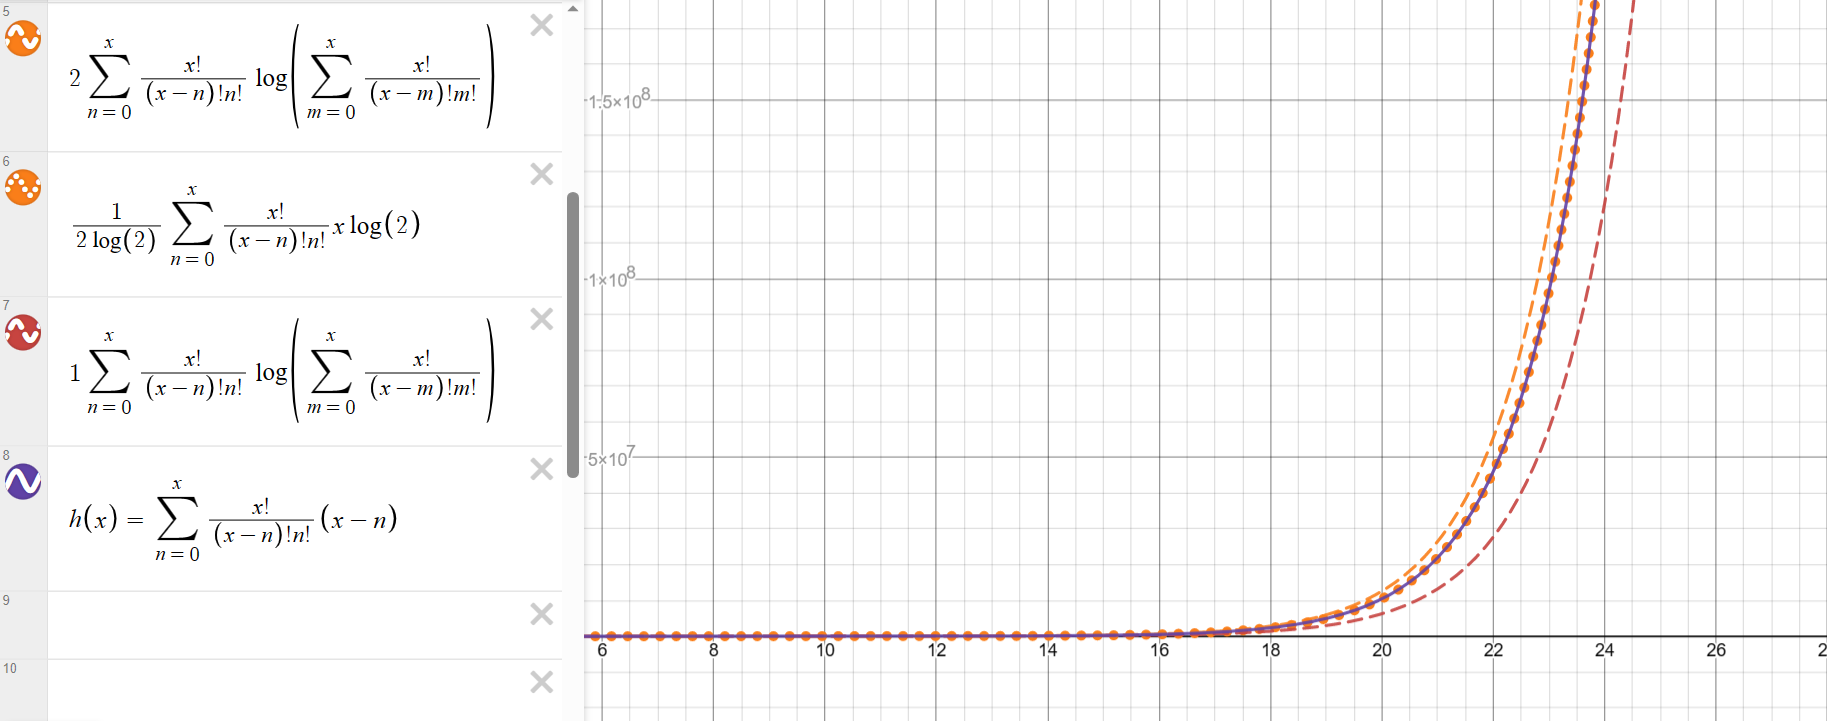
\includegraphics[scale=0.4]{img/DesmosProof.png}
    \caption{The graph demonstrates the proof outlined in this section. Note how three different values of $c$ are demonstrated.}
    \label{fig:DesmosProof}
\end{figure}

\section{Big $\Theta$: Attempting A Geometrical Approach}
\label{sec:TigherBoundGeometricalApproach}

If equation \ref{eq:TotalNumNodesPowerSet} is substituted in the inequalities in equation \ref{eq:nlognInequality}, they can be simplified to equation \ref{eq:nlognInequalityPartiallySimplified}.

\begin{equation}
    \begin{split}
        \forall n_t\ge n_o \;\; &
        c_1|S|\sum_{i=0}^{|S|}\frac{|S|!}{(|S|-i)!i!}
        \log \left( 2 \right)
        \le
        \sum_{i=0}^{|S|}\frac{|S|!}{(|S|-i)!i!}(|S|-i)
        \\
        \forall n_t\ge n_o \;\; &
        \sum_{i=0}^{|S|}\frac{|S|!}{(|S|-i)!i!}(|S|-i)
        \le
        c_2|S|\sum_{i=0}^{|S|}\frac{|S|!}{(|S|-i)!i!}
        \log \left( 2 \right)
    \end{split}
    \label{eq:nlognInequalityPartiallySimplified}
\end{equation}

If analysis similar to what was done in section \ref{sec:UpperBound} is applied to this set of inequalities some surprising results can be had. Similar to section \ref{sec:UpperBound}, if equation \ref{eq:looseInequalities} is true then so must be equation \ref{eq:nlognInequalityPartiallySimplified}.

\begin{equation}
	\begin{split}
		\forall i \;\; & c_1|S|\log(2)\le |S|-i \\
		\forall i \;\; & |S|-i\le c_2|S|\log(2)
	\end{split}
	\label{eq:looseInequalities}
\end{equation}

The second inequality in equation \ref{eq:looseInequalities} is simple enough. $|S|-i$ will be its largest when $i=0$. If the RHS of the second inequality is larger than the LHS's largest value then the inequality is true. Setting $i=0$ and simplifying results in the below inequality.

\begin{equation}
	c_2\ge \frac{1}{\log(2)}
	\label{eq:looseUpperInequality}
\end{equation}

This may seem shocking, equation \ref{eq:looseUpperInequality} does not exactly match the result of equation \ref{eq:BoundaryInequalities}. This is easily explained by simplifying the problem to only consider the largest value of $|S|-i$, instead of the total summation of the $|S|-i$ term.

Following the same logic for the first inequality in equation \ref{eq:looseInequalities} leads to some problems. This time, $|S|-i$ will be its smallest when $i=|S|$. If the LHS of the first inequality is smaller than the RHS's smallest value then the inequality is true. Setting $i=|S|$ and simplifying results in $c_1\le0$, which cannot be the case. This likely seems worse than the previous result, as this time the new way of thinking about the problem resulted in an opposing conclusion. However, this is again easily explained by simplifying the problem to only consider the smallest value of $|S|-i$, instead of the total summation of the $|S|-i$ term. \footnote{On a more positive note, these results show that the result from section \ref{sec:TightBound} truly is a tight bound, as it is not something that can be easily proven for all $i$ values and instead requires careful consideration of the total summation values.}

To consider the total summation value, a more geometric approach is required. Looking at the inequalities shown in equation \ref{eq:looseInequalities}, they can be reinterpreted as representing areas. The $|S|-i$ term represent the area of a triangle with base and height of $|S|$, and the $c_X|S|\log(2)$ term resents the area of a square with sides of length $|S|$ that are scaled by some constant value, $c_X$. With these geometrical interpretations, the inequalities in equation \ref{eq:looseInequalities} can be rewritten as shown in equation \ref{eq:looseInequalitiesArea}.

\begin{equation}
	\begin{split}
		c_1|S|^2\log(2)\le \frac{|S|^2}{2} \\
		\frac{|S|^2}{2}\le c_2|S|^2\log(2)
	\end{split}
	\label{eq:looseInequalitiesArea}
\end{equation}

After simplification the results for the constants match those shown in equation \ref{eq:BoundaryInequalities}. However, there is one small nuance: with this new approach the inequalities were rewritten without the $\forall i$ term because all $i$ values are being the considered through means of the total area. However, removing the $\forall i$ term invalidated the claim that if the inequalities in equation \ref{eq:looseInequalities} were true then the inequalities in equation \ref{eq:nlognInequalityPartiallySimplified} were true because all the values in the inequalities from equation \ref{eq:looseInequalities} were multiplied by $n_c(i)$ within the summations of equation \ref{eq:nlognInequalityPartiallySimplified}. Yet, the result is the exact same as the result from section \ref{sec:TightBound}. This has the following baffling intuition: the summation of the product of the parts is equal to the product of the summations. Or, in more mathematical terms, it implies the following falsehoods to be true:

\begin{equation}
	\begin{split}
		\sum_{i=0}^{|S|}\frac{|S|!}{(|S|-i)!i!}\left(|S| -i\right)
		&\ne
		\left( \sum_{i=0}^{|S|}\frac{|S|!}{(|S|-i)!i!} \right)\sum_{i=0}^{|S|}\left(|S| -i\right)
		\\
		&=
		\left( \sum_{i=0}^{|S|}\frac{|S|!}{(|S|-i)!i!} \right)\frac{|S|^2}{2}
		\\
		\sum_{i=0}^{|S|}\frac{|S|!}{(|S|-i)!i!}
        \log \left( \sum_{j=0}^{|S|-1}\frac{|S|!}{(|S|-j)!j!} \right)
        &\ne
        \left( \sum_{i=0}^{|S|}\frac{|S|!}{(|S|-i)!i!} \right)
        \sum_{i=0}^{|S|}
        \log \left( \sum_{j=0}^{|S|}\frac{|S|!}{(|S|-j)!j!} \right)
        \\
        &=
        \left( \sum_{i=0}^{|S|}\frac{|S|!}{(|S|-i)!i!} \right)
        |S|^2\log(2)
	\end{split}
\end{equation}

There must exist a reason the results match despite the above mathematical falsies. The reason simply boils down to the incorrect removal of the $\forall i$ qualifier in the inequalities listed in equation \ref{eq:looseInequalities}. By removing that qualifier the summations were effectively separated and an extra $|S|$ term was added. The only reason the result of the geometrical approach outlined in this section matched analytical approach outlined in section \ref{sec:TightBound} is because the $|S|$ term was added to both sides of the inequalities, allowing them to cancel out. With that conclusion, this section showed an attempted, but ultimately incorrect, geometrical approach to apply a tight bound.


\section{Asymptotic Behavior and L'Hopital's Rule}
\label{sec:LHopitalsRule}

Another alternative approach that leads to some interesting conclusions is outlined in this section. Imagine trying to prove the following inequality true. It should be clear this inequality is equivalent to the second inequality listed in equation \ref{eq:looseInequalities}.

\begin{equation}
	\begin{split}
		\forall i \;\; |S|-i\le c_2 \log \left( \sum_{j=0}^{|S|}\frac{|S|!}{(|S|-j)!j!} \right)
	\end{split}
	\label{eq:singleInequality}
\end{equation}

To simplify the inequality a different approach will be used. Instead of considering the entire summation, only the largest value of the summation will be considered. \footnote{This is also why one one inequality is being considered. Proving that $|S|-i$ is greater than the largest value of the summation does nothing to prove it is greater than the entire summation.} If the inequality can be proven for this smaller value then it should also be true for the entire summation. Given the combinatoric nature of the summation, it should be obvious that the largest value will occur when $j=\frac{|S|}{2}$. This makes the new inequality take the form shown in equation \ref{eq:singleInequalitySingleSumValue}.

\begin{equation}
	\begin{split}
		\forall i \;\; |S|-i\le c_2 \log \left( \frac{|S|!}{(|S|-\frac{|S|}{2})!\frac{|S|}{2}!} \right)
	\end{split}
	\label{eq:singleInequalitySingleSumValue}
\end{equation}


%To find the largest value, the range of $j$ must be considered, which is $0\to |S|$. Replacing $j$ with equation \ref{eq:} will let the summation values be treated as continuous and classical calculus can be used to find the maximum value.

%\begin{equation}
%	j=k|S|\text{ where }0\le k\le |S|
%\end{equation}

The nature of the above inequality is not entirely visible, so it might help to just focus on the asymptotic behavior of the inequality. This is ok because any time complexity is also concerned with asymptotic behavior. In order to do this L'Hopital's rule is required.

\begin{equation*}
	\begin{split}
		\lim_{|S|\to \infty} \frac{
			\frac{d}{d|S|}				
			c \log \left( \frac{
				|S|!
			}{
				\left(|S|-\frac{|S|}{2}!\right)!\frac{|S|}{2}!
			} \right)
		}{
			\frac{d}{d|S|}
			|S|-i
		}
		= &
		\lim_{|S|\to \infty} \frac{
			c \frac{d}{d|S|}				
			\log \left( |S|! \right)-2\log \left( \frac{|S|}{2}! \right)
		}{
			1
		}
		\\
		= &
		\lim_{|S|\to \infty}
		c \frac{d}{d|S|}				
		\log \left( \prod_{k=1}^{|S|} k \right)-2\log \left( \prod_{k=1}^{\frac{|S|}{2}} k \right)
		\\
		= &
		c \lim_{|S|\to \infty}
		\frac{d}{d|S|}
		\sum_{k=1}^{|S|}\log(k)-2\sum_{k=1}^{\frac{|S|}{2}}\log(k)
	\end{split}
\end{equation*}

At this point the math gets a little difficult due to the variable of differentiation being in the summation boundaries. To progress past this point the summations will be approximated with an integral.

\begin{equation*}
	\begin{split}
		c \lim_{|S|\to \infty} &
		\frac{d}{d|S|}
		\sum_{k=1}^{|S|}\log(k)-2\sum_{k=1}^{\frac{|S|}{2}}\log(k)
		\approx
		\lim_{|S|\to \infty}
		\frac{d}{d|S|}
		\int_{k=1}^{|S|}\log(k)\,dk-2\int_{k=1}^{\frac{|S|}{2}}\log(k)\,dk
		\\		
		= &
		c \lim_{|S|\to \infty}
		\left(
			\log(|S|)(1)-\log(1)(0)
		\right)-2\left(
			\log\left( \frac{|S|}{2}	\right)\left( \frac{1}{2} \right)-\log(1)(0)
		\right)
		\\
		= &
		c \lim_{|S|\to \infty}
		\log(|S|)-\log\left(\frac{|S|}{2}\right)
		\\
		= &
		c \lim_{|S|\to \infty}
		\log(2)=\log(2)
	\end{split}
\end{equation*}

Given this result the inequality shown in equation \ref{eq:singleInequalitySingleSumValue} holds true, and it can be said that the number of items in the set grows less than or equal to the number of nodes times the log of the number of nodes, or $e_t\in O(n_tlog(n_t))$. This is a subset of the results gained in section \ref{sec:TightBound}. It is tempting to say this result makes sense because it matches the results gained from section \ref{sec:TightBound}, but it is worth remembering that we only considered the largest value of the summation. Despite only considering the largest value of the summation, we still got the same growth rate as the entire summation. In mathematical terms, it would be saying the following fallacy is true.

\begin{equation*}
	\begin{split}
		\frac{d}{d|S|}				
		\log \left( \frac{
			|S|!
		}{
			\left(|S|-\frac{|S|}{2}!\right)!\frac{|S|}{2}!
		} \right)
		= &
		\log(2)
		\\
		\frac{d}{d|S|}				
		\log \left( \sum_{j=0}^{|S|} \frac{
			|S|!
		}{
			\left(|S|-j!\right)!j!
		} \right)
		= &
		\frac{d}{d|S|} |S|\log(2)=\log(2)
		\\
		\therefore  \;\;
		\frac{d}{d|S|}				
		\log \left( \frac{
			|S|!
		}{
			\left(|S|-\frac{|S|}{2}!\right)!\frac{|S|}{2}!
		} \right)
		= &
		\frac{d}{d|S|}				
		\log \left( \sum_{j=0}^{|S|} \frac{
			|S|!
		}{
			\left(|S|-j!\right)!j!
		} \right)
		=\log(2)
	\end{split}	
\end{equation*}

This obviously cannot be true. The reason for this incorrect result can be traced back to approximating the summations with an integral. To understand this error better it can be approximated. Imagine the error as the summation of a bunch of triangles where each triangle represents the extra area from each summation value. This triangle will have a width of $1$ and a height equal to the difference of the current and previous summation values. This idea is shown in figure \ref{fig:LogApprox} for better understanding. Also note that the smallest value from the summations is $2$, meaning the error related to the negative portion of $\log(k)$ does not need to be considered. This error term is not exact, but including it will give better results than if it were not included.

\begin{figure}[h]
    \center
    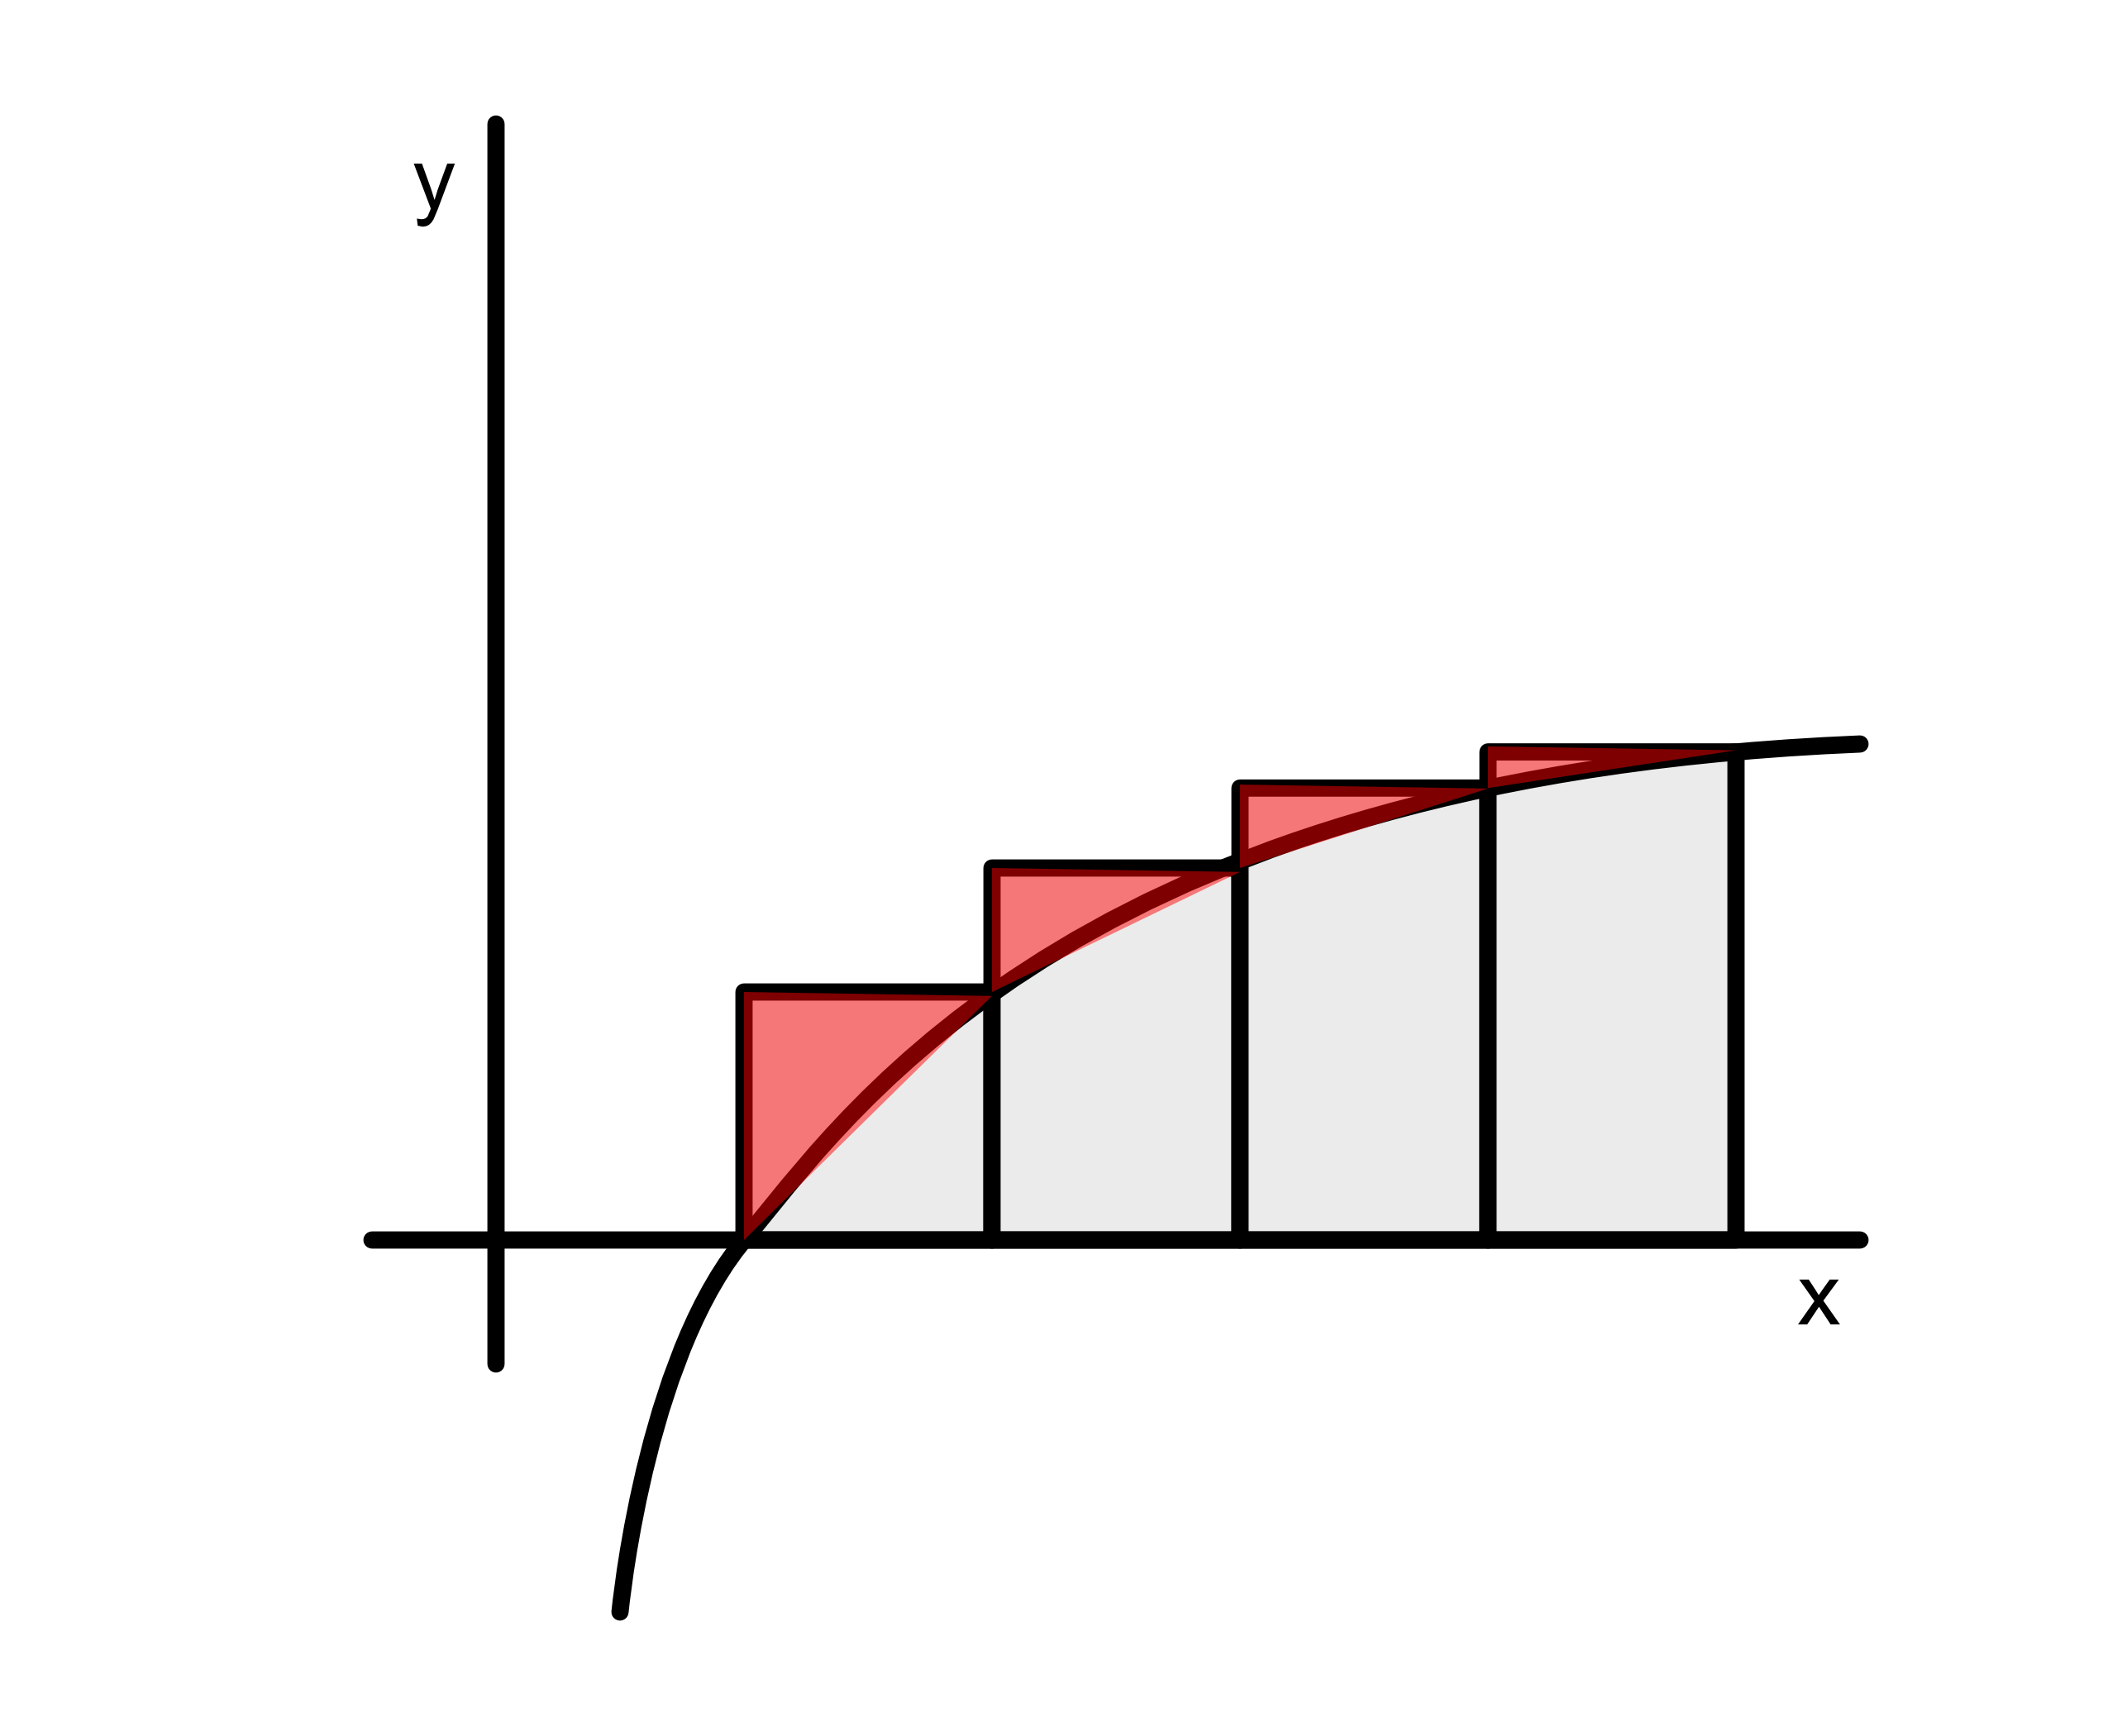
\includegraphics[scale=0.4]{img/LogApprox.png}
    \caption{A graphical representation of the error of approximating the summation of $log(x)$ with an integral. Note that this graph is not an actual graph of log, just a picture to help convey an idea.}
    \label{fig:LogApprox}
\end{figure}

Mathematically the same idea is represented in equation \ref{eq:BetterApprox}. Note how the error term is not bounded, or put in other words the error will not approach a single value as $N$ increases. This means the approximation made before which did not account for this error only got more and more wrong as $N\to \infty$. Given that the goal was to perform asymptotic analysis, this presents an obvious problem. Graphically, the effects of this  error term are demonstrated in figure \ref{fig:DesmosErrProof}.


\begin{equation}
	\begin{split}
		\sum_{i=1}^N \log(i)
		\approx &
		\int_{1}^N \log(i) \,di+\sum_{i=2}^N \frac{1}{2}(\log(i)-\log(i-1))
		\\
		= &
		\int_{1}^N \log(i) \,di+\frac{1}{2} \sum_{i=2}^N \log\left(\frac{i}{i-1}\right)
		\\
		= &
		\int_{1}^N \log(i) \,di+\frac{1}{2} \log\left( \prod_{i=2}^N \frac{i}{i-1} \right)
		\\
		= &
		\int_{1}^N \log(i) \,di+\frac{1}{2} \log\left( N \right)
		\\
		\text{or}
		\\
		\sum_{i=1}^{N-1} \log(i)
		\approx &
		\int_{1}^N \log(i) \,di-\frac{1}{2} \log\left( N \right)
		\\
		\text{or}
		\\
		\int_{1}^N \log(i) \,di
		\approx &
		\sum_{i=1}^N \log(i)-\frac{1}{2}\log(N)
		\\
		\text{or}
		\\
		\int_{1}^N \log(i) \,di
		\approx &
		\sum_{i=1}^{N-1} \log(i)+\frac{1}{2}\log(N)
	\end{split}
	\label{eq:BetterApprox}
\end{equation}

\begin{figure}[h]
    \center
    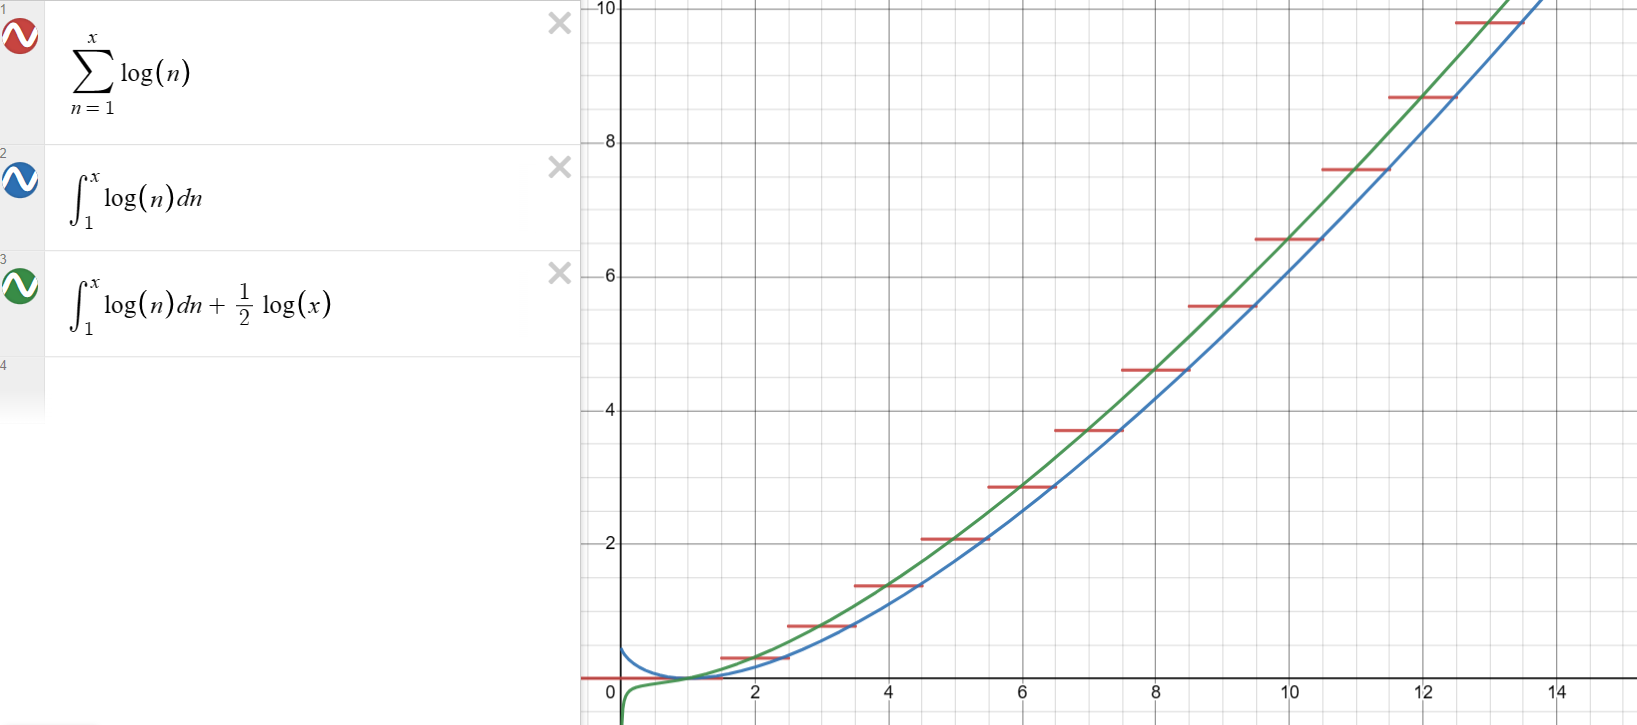
\includegraphics[scale=0.4]{img/DesmosLogErrProof.png}
    \caption{A graph showing how the error term better matches the summation's values.}
    \label{fig:DesmosErrProof}
\end{figure}

Given this better approximation, the next natural question is if it can be used to garnish the correct result. The same approximation made before is shown below with the new error term.

\begin{equation}
	\begin{split}
		c \lim_{|S|\to \infty} &
		\frac{d}{d|S|}
		\sum_{k=1}^{|S|}\log(k)-2\sum_{k=1}^{\frac{|S|}{2}}\log(k)
		\\
		\approx
		c \lim_{|S|\to \infty} &
		\frac{d}{d|S|}
		\left( 
			\int_{k=1}^{|S|}\log(k)\, dk
			+
			\frac{1}{2}\log(|S|)
		\right) - 2\left( 
			\int_{k=1}^{\frac{|S|}{2}}\log(k) \,dk
			+
			\frac{1}{2}\log\left( \frac{|S|}{2} \right)
		\right)
		\\
		=
		c \lim_{|S|\to \infty} &
		\left(
			\log(|S|)(1)-\log(1)(0)
		\right)
		+\frac{1}{2|S|}		
		-2\left(
			\log\left( \frac{|S|}{2} \right)\left( \frac{1}{2} \right)-\log(1)(0)
		\right) - \frac{1}{|S|}
		\\
		=
		c \lim_{|S|\to \infty} &
		\log(|S|)-\log\left( \frac{|S|}{2} \right)-\frac{1}{2|S|} = 
		\log(2)
	\end{split}
\end{equation}

By including the error terms the growth rates of the entire summation and the largest value of the summation no longer match, as would be expected. Of note is that the final answer was the same. Applying L'Hopital's rule to both approximations reached the final answer of $\log(2)$, creating the inequality shown in equation \ref{eq:Missing2BoundaryInequalities}.

\begin{equation*}
	\begin{split}
		\frac{d}{d|S|}				
		\log \left( \frac{
			|S|!
		}{
			\left(|S|-\frac{|S|}{2}!\right)!\frac{|S|}{2}!
		} \right)
		= &
		\log(2)-\frac{1}{2|S|}
		\\
		\frac{d}{d|S|}				
		\log \left( \sum_{j=0}^{|S|} \frac{
			|S|!
		}{
			\left(|S|-j!\right)!j!
		} \right)
		= &
		\frac{d}{d|S|} |S|\log(2)=\log(2)
		\\
		\therefore  \;\;
		\frac{d}{d|S|}				
		\log \left( \frac{
			|S|!
		}{
			\left(|S|-\frac{|S|}{2}!\right)!\frac{|S|}{2}!
		} \right)
		\ne &
		\frac{d}{d|S|}				
		\log \left( \sum_{j=0}^{|S|} \frac{
			|S|!
		}{
			\left(|S|-j!\right)!j!
		} \right)
	\end{split}	
\end{equation*}

\begin{equation}
	\begin{split}
        c_2 &\ge \frac{1}{\log(2)}
	\end{split}
	\label{eq:Missing2BoundaryInequalities}
\end{equation}

Similar to the results in section \ref{sec:TigherBoundGeometricalApproach}, the inequality listed in equation \ref{eq:Missing2BoundaryInequalities} does not match the correct inequalities from equation \ref{eq:BoundaryInequalities}. The reason for this is two fold:

\begin{enumerate}
	\item This section only considered the inner summations of the inequalities in equation \ref{eq:nlognInequality}.
	\item This section was concerned with asymptotic behavior.
\end{enumerate}

Of note is that the value for $c_2$ found in this section is still valid, it is just a looser bound than the one found in section \ref{sec:TightBound}. This is also reflected in only being able to prove big-O in this section instead of matching the big-$\Theta$ from section \ref{sec:TightBound}.

\begin{equation*}
	\frac{1}{2\log(2)}<\frac{1}{\log(2)}
\end{equation*}

\section{Actually Visiting The Edges}
\label{sec:VisitingEdges}

So it has been proven that the total number of edges grows with respect to the total number of nodes multiplied by the log of the total number of nodes, or $e_t\in \Theta(n_t\log(n_t))$s. This is great, but how can the edges \textit{actually be traversed} in such a way that every edge is only visited once.

Now that we have ways of expressing the number of nodes and edges in this DAG we are traversing, the question remains how to visit every edge in this graph
where backtracking is not allowed. More specifically, what is the minimum
number of times you must restart at the start node (the top element of the
lattice if you will) and traverse along paths in the graph until you have
visited every edge? This is equivalent to the well known minimum path cover
problem.  TODO Can we prove that the minimum path cover is equal to the number
of edges coming out of the largest column? Idk, it certainly feels correct.
Maybe use max cut/min flow theorem? Also, is Kuhn's algorithm ultimately
equivalent to my idea of finding augmenting paths by searching for the closest
parent to the start node with an unvisited edge and extending as far as
possible?  Assume the optimal number of paths in the minimum path cover is
equal to the number of edges coming out of the largest column. How many edges
is this? First lets find how many nodes are in the largest column.
$$s = |S|$$
$$n_{\frac{s}{2}} = \frac{s!}{(s - \frac{s}{2})!(\frac{s}{2})!} = \frac{s!}{\frac{s}{2}!^2}$$
Use stirling's approximation $n! = O(n^n\sqrt{n})$
$$ = O(\frac{s^s\sqrt{s}}{((\frac{s}{2})^\frac{s}{2}\sqrt{\frac{s}{2}})^2})$$
$$ = O(\frac{s^s\sqrt{s}}{(\frac{s}{2})^s\frac{s}{2}}) = O(2^s\frac{\sqrt{s}}{s}) = O(\frac{2^s}{\sqrt{s}})$$
We also know $e_{\frac{s}{2}} = n_{\frac{s}{2}}\frac{s}{2}$
$$e_{\frac{s}{2}} = O(2^s\sqrt{s})$$
This makes sense because the number of nodes in each column represent binomial coefficients which approximate a normal distribution as $s$ approaches infinity. The integral of the normal distribution could be approximated asymptotically with a rectangle with the same height as the mean and width equal to the inflection points. The inflection points of the normal distribution occur at one standard deviation away from the mean. The variance of the normal distribution that these binomial coefficient approach is $\frac{s}{4}$, so linear with respect to s. Therefore the standard deviation, and furthermore the width of our rectangle approximation should grow with $\sqrt{s}$. This means that the height of this rectangle multiplied by $\sqrt{s}$ should be equal to $2^s$.


\section{Appendix A}
\label{ap:A}

Through all the chaos in section \ref{sec:LHopitalsRule} it is easy to overlook one simple geometric intuition. To begin, start with the equation shown below. This equation was the result of the first approximation in section \ref{sec:LHopitalsRule}.

\begin{equation*}
	\frac{d}{d|S|}
	\int_{k=1}^{|S|}\log(k)\,dk-2\int_{k=1}^{\frac{|S|}{2}}\log(k)\,dk
\end{equation*}

After some simplifications, the following equation can be gathered.

\begin{equation*}
	\begin{split}
		\frac{d}{d|S|}
		\int_{k=1}^{|S|}\log(k)\,dk-2\int_{k=1}^{\frac{|S|}{2}}\log(k)\,dk
		= &
		\frac{d}{d|S|}
		\int_{k=\frac{|S|}{2}}^{|S|}\log(k)\,dk-\int_{k=1}^{\frac{|S|}{2}}\log(k)\,dk
		\\
		= &
		\frac{d}{d|S|}
		k\log(k)-k \Big|_{\frac{|S|}{2}}^{|S|}-
		k\log(k)-k \Big|_{1}^{\frac{|S|}{2}}
		\\
		= &
		\frac{d}{d|S|}
		|S|\log(|S|)-|S|
		-|S|\log\left(\frac{|S|}{2}\right)+|S|
		+1\log(1)-1
		\\
		= &
		\frac{d}{d|S|}
		|S|\log(|S|)
		-|S|\log\left( \frac{|S|}{2} \right)
		-1
		\\
		= &
		\log(2)
	\end{split}
\end{equation*}

What this equation says geometrically is quite interesting: the difference of the rate of growth of the areas of the upper and lower half of $\log(x)$ is $\log(2)$. Figure \ref{fig:LogArea} puts this in a more graphical form.

\begin{figure}[h]
    \center
    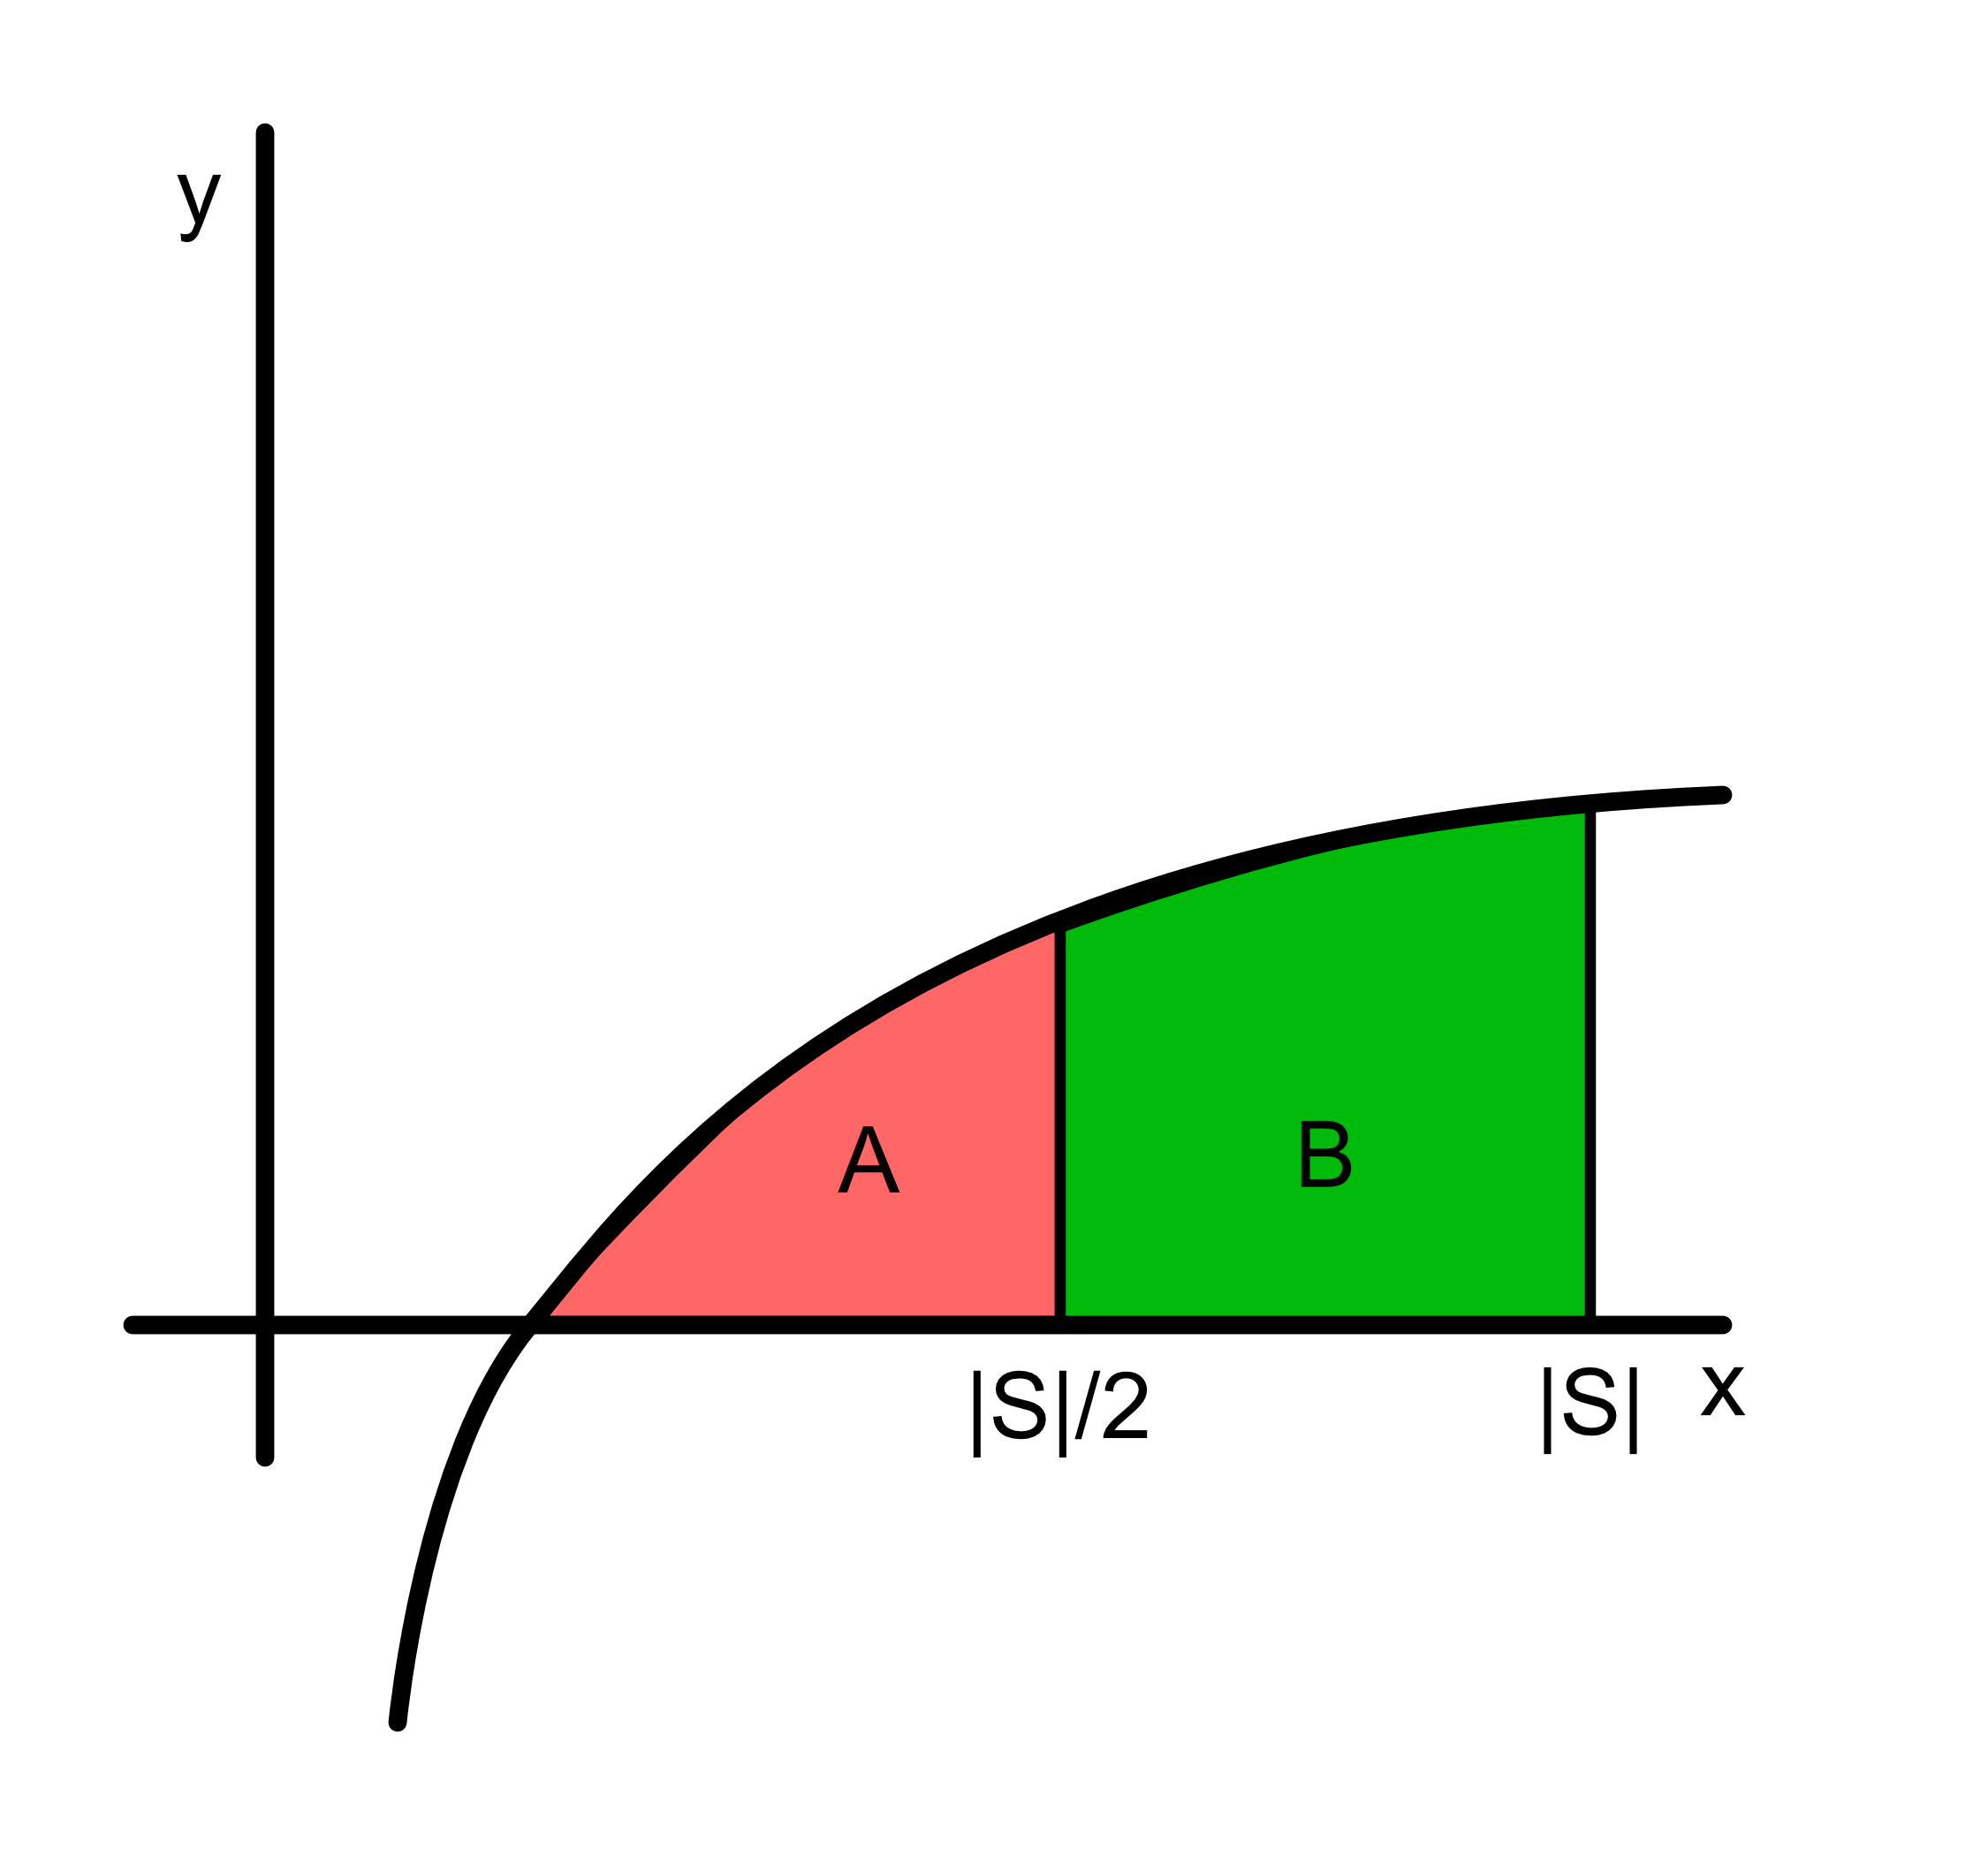
\includegraphics[scale=0.4]{img/LogArea.png}
    \caption{A graph demonstrating the aforementioned geometric intuitions. Note that this graph is not an actual graph of log, just a picture to help convey an idea.}
    \label{fig:LogArea}
\end{figure}

Using the graph, the previous equation can be restated in a possibly more intuitive manner.

\begin{equation}
	\frac{d}{d|S|}(B-A)=\log(2)
\end{equation}


\section{Examples}

\begin{theorem}
    This is a theorem.
\end{theorem}

\begin{proposition}
    This is a proposition.
\end{proposition}

\begin{principle}
    This is a principle.
\end{principle}

% Maybe I need to add one more part: Examples.
% Set style and colour later.

\subsection{Pictures}


\subsection{Citation}

This is a citation\cite{Eg}.

\newpage

% ------------------------------------------------------------------------------
% Reference and Cited Works
% ------------------------------------------------------------------------------

\bibliographystyle{IEEEtran}
\bibliography{References.bib}

% ------------------------------------------------------------------------------

\end{document}
